\section{Typed realizability}
\label{sec:typed-realizability}

RZ is based on \emph{typed realizability} by John
Longley~\cite{Longley99}. It is a variant of realizability that most
directly corresponds to the informal view that a programmer has in
mind when thinking about an implementation of a structure.

We motivate and explain typed realizability and its relationship with
real-world programming by way of example. Suppose we are asked to
design a data structure for the set $\mathcal{G}$ of all finite
simple\footnote{There is at most one arrow between any two vertices.}
directed graphs with vertices labelled by integers. An exemplar
directed graph~$G$ is shown in Figure~\ref{fig:digraph}.
%
\begin{figure}
  \centering
  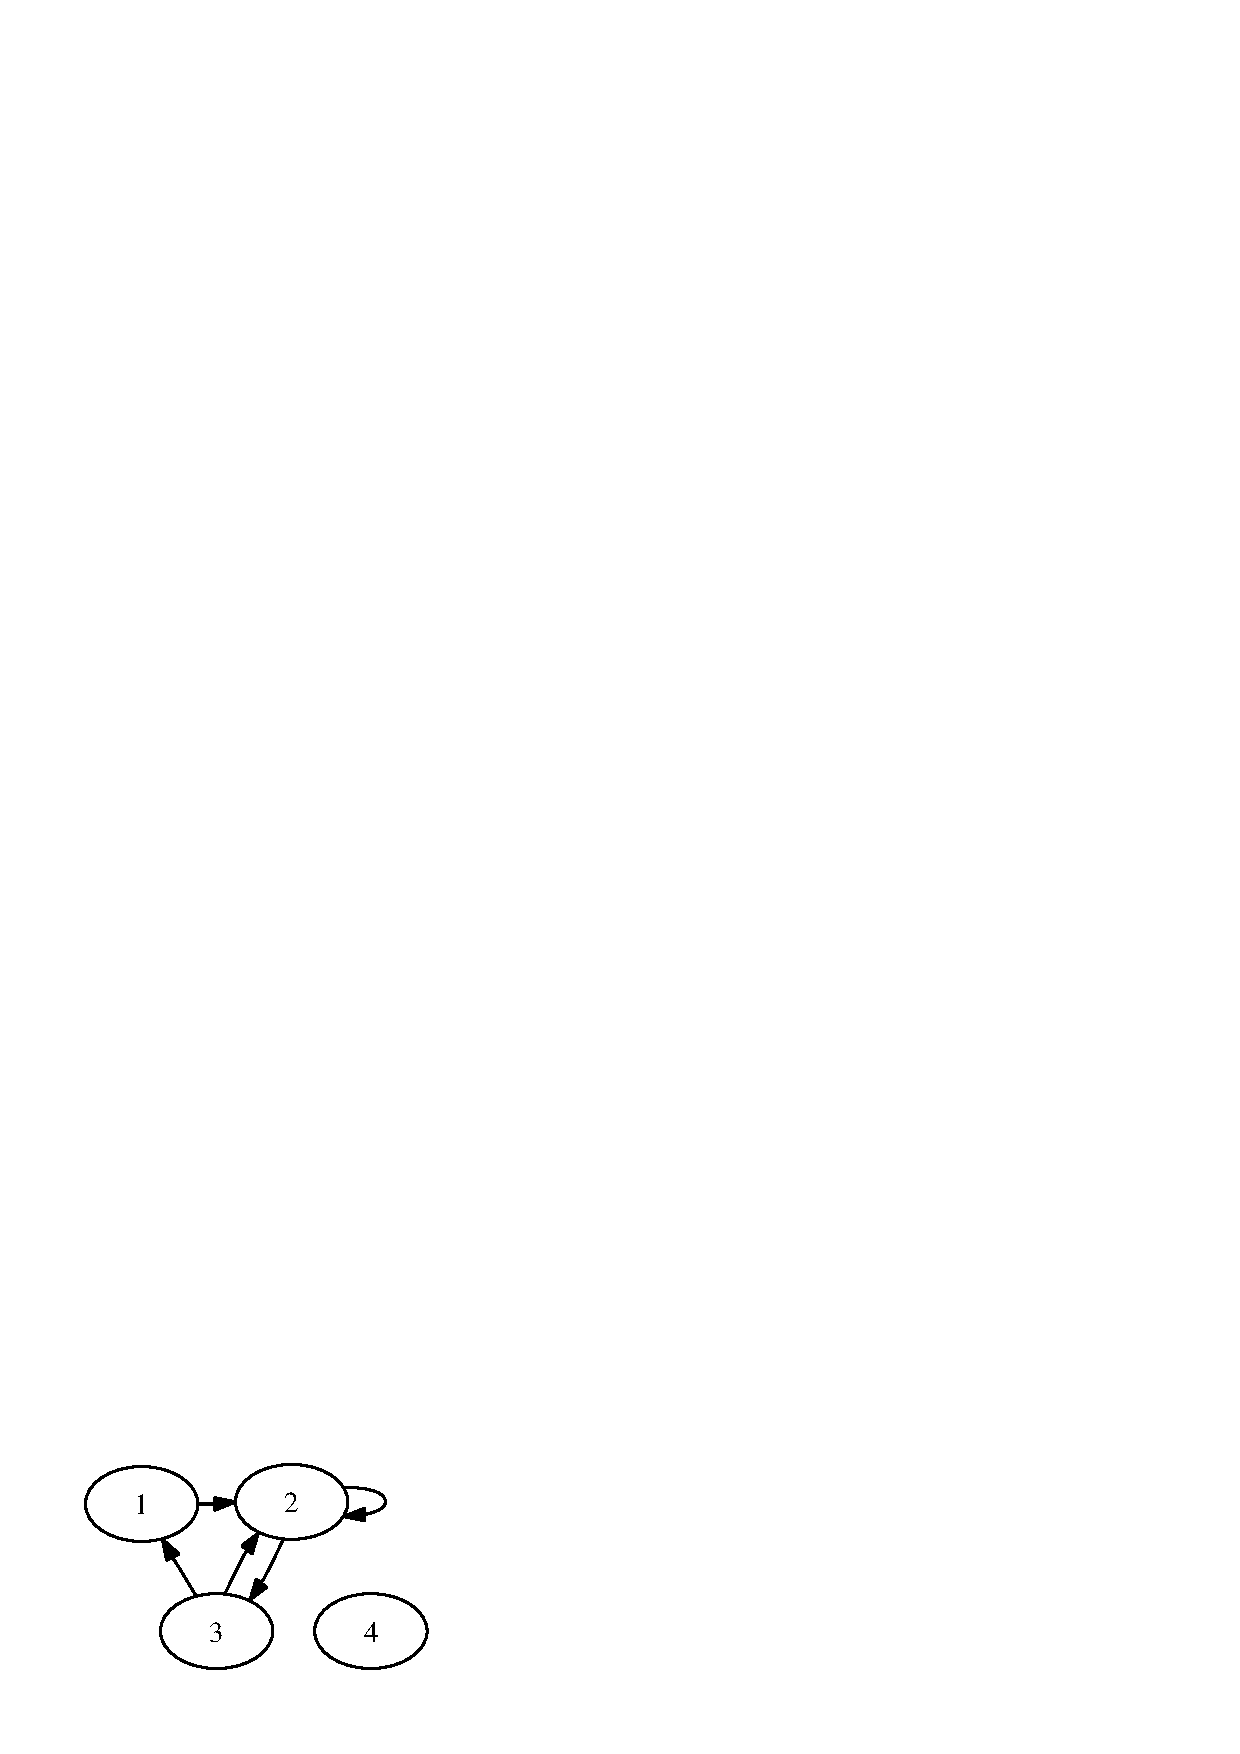
\includegraphics[width=0.4\textwidth]{digraph}
  \caption{A finite directed graph $G$}
  \label{fig:digraph}
\end{figure}
%
A common representation is a pair of lists $(\ell_V, \ell_A)$, where
$\ell_V$ is the list of vertices and $\ell_A$ the list of arrows,
known as the \emph{adjacency list}. In our example, $\ell_V = [1; 2;
3; 4]$ and $\ell_A = [(1,2); (2,2); (2,3); (3,2); (3;1)]$. Thus we
define the datatype of graphs to be\footnote{We use Ocaml notation in
  which $\clist{t}$ means lists of elements of type~$t$, and
  $t_1 * t_2$ means the type of ordered pairs whose first component
  has type $t_1$ and second type $t_2$.}
%
\begin{equation*}
  \ctype \mathtt{graph} = \clist{\cint} * \clist{(\cint * \cint)}
\end{equation*}
%
However, this is not a complete description of the representation, as
there are invariants and conditions which are not expressed directly
in the programming language, such as:
%
\begin{enumerate}
\item The order in which vertices and arrows are listed is not
  important, e.g., $[1;2;3;4]$ and $[4;1;2;3]$ represent the same vertices.
\item Each vertex and arrow must be listed exactly once.
\item Infinite, cyclic lists, and non-terminating expressions are not
  valid representations, e.g.,
  %
  \begin{equation*}
    \cwhile{\ctrue}{()}; [(1,2);(2,2);(2,3);(3,2);(3;1)]
  \end{equation*}
  %
  is not a valid adjacency list, and neither is an expression that
  raises an exception.
\item We ought to decide which computational effects, if any, are
  allowed, e.g., is
  %
  \begin{equation*}
    \cprint{\cstring{Hello}}; [(1,2);(2,2);(2,3);(3,2);(3;1)]
  \end{equation*}
  %
  a valid adjacency list?
\end{enumerate}
%
To summarize, an implementation of the set~$\mathcal{G}$ should tell
us not only what the underlying datatype $\mathtt{graph}$ is, but also
which values of type $\mathtt{graph}$ represent which elements
of~$\mathcal{G}$. As we shall see next, all of this can be expressed
either as a \emph{realizability relation} or a \emph{partial
  equivalence relation (per)}.


\subsection{Modest sets and pers}
\label{sec:modest-sets-pers}

We now give the formal definition of typed realizability, as it
applies to Ocaml. Other general-purpose programming languages could be
used instead, as long as they provide the usual ground types, product
and function types. Additionally, it is convenient to work with a
language that supports sum types, as this allows a more natural
representation of disjoint unions.

Let $\Type$ be the collection of all (non-parametric) Ocaml types. To
each type $t \in \Type$ we assign the set $\values{t}$ of values of
type~$t$ which behave \emph{functionally} in the sense
of~\cite{longley99when}. Such values are represented by terminating
expressions which do not raise exceptions or return different results
on different invocations, although they \emph{may} use exceptions,
store, and other computational effects, as long as they behave as if
they did not. A useful example of a functional value using store is
presented in Section~\ref{sec:we-show-modulus-of-continuity-example}.
Note also that a functional value of a functional type may diverge as
soon as it is applied, e.g., if we define
$\cletrec{f\;(x:\cint):\cint}{f\;x}$ then $f \in \values{\cint \to
  \cint}$. The collection $\Type$ with the assignment of functional
values $|t|$ to each $t \in \Type$ forms a \emph{typed partial
  combinatory algebra (TPCA)}, which provides a theoretical basis for
the definition of a realizability model that suits our needs.

Going back to our example, we see that to implement the set of
directed graphs $\mathcal{G}$ is to specify a datatype
$\typeOf{\mathcal{G}} = \mathtt{graph}$ together with a
\emph{realizability relation} $\rz_{\mathcal{G}}$ between
$\mathcal{G}$ and $\values{\mathtt{graph}}$. The meaning of $(\ell_V,
\ell_A) \rz_\mathcal{G} G$ is ``value $(\ell_V, \ell_A)$ represents
(realizes, implements) graph $G$''. There are two natural conditions
that $\rz_\mathcal{G}$ ought to satisfy: (1) for every $G \in
\mathcal{G}$ there should be at least one realizer $(\ell_V, \ell_A)$
representing it, and (2) if $(\ell_V, \ell_A)$ represents both $G$ and
$G'$ then $G = G'$. The latter condition is called \emph{modesty} and
is not strictly necessary for the development of the theory, though it
is something that programmers would naturally expect to hold. If
$(\ell_V, \ell_A)$ and $(\ell'_V, \ell'_A)$ represent the same graph,
we say that they are \emph{equivalent} and write $(\ell_V, \ell_A)
\per_\mathcal{G} (\ell'_V, \ell'_A)$. The relation $\per_\mathcal{G}$
is a \emph{partial} equivalence relation (symmetric and transitive,
but not reflexive) because not every $(\ell_V, \ell_A) \in
\values{\mathtt{graph}}$ represents a graph.

\bigskip

A general definition is in order. A \emph{modest set} is a triple $A =
(\setOf{A}, \typeOf{A}, {\rz_A})$ where $\setOf{A}$ is the
\emph{underlying set}, $\typeOf{A} \in \Type$ is the \emph{underlying
  type}, and $\rz_A$ is a \emph{realizability relation} between
$\values{\typeOf{A}}$ and $\setOf{A}$, satisfying
% 
\begin{enumerate}
\item \emph{totality:} for every $x \in \setOf{A}$ there is $v \in
  \typeOf{A}$ such that $v \rz_A x$, and
\item \emph{modesty:} if $u \rz_A x$ and $u \rz_A y$ then $x = y$.
\end{enumerate}
%
The \emph{support} of $A$ is the set $\support{A} = \set{v \in
  \typeOf{A} \such \xsome{x}{\setOf{A}}{v \rz_A x}}$ of those values
which realize something. We define the relation $\per_A$ on
$\values{\typeOf{A}}$ by
%
\begin{equation*}
  u \per_A v
  \iff
  \some{x}{\setOf{A}}{u \rz_A x \land v \rz_A x} \;.
\end{equation*}
%
From totality and modesty of $\rz_A$ it follows that $\rz_A$ is a per,
i.e., symmetric and transitive. Observe that $\support{A} = \set{v \in
  \values{\typeOf{A}} \such v \per_A v}$, whence $\per_A$
restricted to $\support{A}$ is an equivalence relation. In fact, we
may recover a modest set up to isomorphism from $\typeOf{A}$ and
$\per_A$ by taking $\setOf{A}$ to be the set of equivalence classes of
$\per_A$, and $v \rz_A x$ to mean $v \in x$.

The two views of implementations, as modest sets $(\setOf{A},
\typeOf{A}, {\rz_A})$, and as pers $(\typeOf{A}, {\per_A})$, are
equivalent. In RZ we use pers because they refer only to types and
values, as opposed to arbitrary sets. Nevertheless, it is useful to
understand how modest sets and pers arise from natural considerations
about programming practice.

Modest sets form a category whose objects are modest sets and
morphisms are the realized functions. A \emph{realized function} $f :
A \to B$ is a function $f : \setOf{A} \to \setOf{B}$ such that there
exists $v \in \values{\typeOf{A} \to \typeOf{B}}$ for which
%
\begin{equation}
  \label{eq:rz-function-space}
  \xall{x}{\setOf{A}}{
    \all{u}{\typeOf{A}}{
      u \rz_A x \implies v\;u \rz_B f(x)
    }
  }.
\end{equation}
%
This condition is just a mathematical expression of the usual idea
that~$v$ is an implementation of~$f$, since~$v$ does to realizers
what~$f$ does to the elements they represent.

The equivalent category of pers has as objects pairs $A = (\typeOf{A},
{\per_A})$ where $\typeOf{A} \in \Type$ and $\per_A$ is a per on
$\values{\typeOf{A}}$. A morphism $A \to B$ is represented by $v
\in \values{\typeOf{A} \to \typeOf{B}}$ such that, for all $u, u'
\in \support{A}$,
%
\begin{equation}
  \label{eq:per-exponential}
  u \per_A u' \implies v\;u \per_B v\;u' \;.
\end{equation}
%
Values $v$ and $v'$ which both satisfy~\eqref{eq:per-exponential}
represent the same morphism if, for all $u, u' \in \support{A}$,
%
\begin{equation*}
  u \per_A u' \implies v\;u \per_B v'\;u' \;.
\end{equation*}

The category of modest sets has a very rich structure. For example, we
may form a cartesian product $A \times B$ of modest sets $A$ and $B$
by
%
\begin{align*}
  \setOf{A \times B} &= \setOf{A} \times \setOf{B},\\
  \typeOf{A \times B} &= \typeOf{A} * \typeOf{B},\\
  p \rz_{A \times B} (x,y) &\iff
  \cfst{p} \rz_A x \land csnd{p} \rz_B y.
\end{align*}
%
The projections $\pi_1 : A \times B \to A$ and $\pi_2 : A \times B \to
B$ are realized by $\cfun{p}{\cfst{p}}$ and $\cfun{p}{\csnd{p}}$,
respectively.

The morphisms between modest sets~$A$ and~$B$ again form a modest set
$B^A$, also written as $A \to B$, called the \emph{exponential} of~$A$
and~$B$, with the underlying set
%
\begin{equation*}
  \setOf{B^A} =
  \set{f : \setOf{A} \to \setOf{B} \such \text{$f$ is a realized function}},
\end{equation*}
%
the underlying type
%
\begin{equation*}
  \typeOf{B^A} = \typeOf{A} \to \typeOf{B},
\end{equation*}
%
and the realizability relation $\rz_{B^A}$ defined
by~\eqref{eq:rz-function-space}. The evaluation map $e : B^A \times A
\to B$, $e(f,x) = f(x)$ is realized by $\cfun{(u,v)}{u\;v}$. If a
function $f : C \times A \to B$ is realized by $v$, then its transpose
$\tilde{f} : C \to B^A$, $\tilde{f}(z)(x) = f(z,x)$, is realized by
$\cfun{z\;x}{v \; (z,x)}$. This shows that the category of modest sets
is cartesian closed. In Section~\ref{sec:realizability-interpretation}
we review other canonical constructions on modest sets, such as
products and sums.

\subsection{Two Examples}
\label{sec:examples-modest-sets}

As a first example we implement the cyclic group on seven elements
$(\ZZ_7, 0, {-}, {+})$. For the implementation we must give a
representation of $\ZZ_7$ as a modest set~$Z = (\ZZ_7, \typeOf{Z},
{\rz_Z})$, and show that negation $-$ and addition $+$ are realized.
We represent the elements of~$\ZZ_7 = \set{0, 1, \ldots, 6}$ with
values of type $\typeOf{Z} = \cint$ and the realizability relation
%
\begin{equation*}
  v \rz_Z k \iff v = k \;.
\end{equation*}
%
This says that $v \in \values{\cint}$ represents an element $k \in
\ZZ_7$ if it is equal to it. The associated per is
%
\begin{equation*}
  u \per_Z v
  \iff
  0 \leq u = v \leq 6 \;.
\end{equation*}
%
Negation is realized by the function $\mathtt{neg}: \cint \to \cint$,
%
\begin{equation*}
  \clet{\mathtt{neg}\; k}{7 - k},
\end{equation*}
%
while addition is realized by $\mathtt{add}: \cint * \cint \to \cint$,
%
\begin{equation*}
  \clet{\mathtt{add}\;(k,m)}{(k + m) \;\mathtt{mod}\; 7}\;.
\end{equation*}
%
The modest set~$Z$ also has \emph{decidable equality}, which means
that the characteristic map $\mathrm{eq} : Z \times Z \to
\set{\mathtt{false}, \mathtt{true}}$ of equality is realized, namely
by $\cfun{(k,m)}{(k=m)}$. However, not all modest sets have decidable
equality, since there may not be a decision procedure for determining
whether two realizers represent the same element. In particular, this
would happen if we implemented a group with an undecidable word
problem~\cite{undecidable-word-problem}.


\internal{AB}{Example: Natural numbers. Explicitly postulate the
  realizer for induction, using the type $\alpha \to (\alpha \to
  \alpha) \to \mathtt{nat} \to \mathtt{\alpha}$ of a realizer for
  induction.}


\subsection{Uniform families}
\label{sec:uniform-families}

Give an example of a uniform family (probably the cyclic group of rank
$n$).

Describe uniform families and mention that they are related to
dependent types. Motivate and discuss the uniformity. Describe the
dependent sums and products.


%%% Local Variables: 
%%% mode: latex
%%% TeX-master: "cie"
%%% End: 
